
\section{Introducing Java}
\label{sec:introducing-java}

The time has come to start using full-flavoured Java. This section
will introduce the main features that are new with respect to what we
have seen so far. We will make a gradual transition to the new
language. 

\subsection{Everything is a class}
\label{sec:everything-class}

In Java all the code comes inside a class. There is no class-less
code as in Groovy. 

Usually every class is defined in its own file, e.g.~a \verb+Person+
class is defined in a file called \verb+Person.java+. When a file
contains only one class, this class must be public and have the same
name as the file (without the \verb+.java+ extension). 

Classes in different files must be compiled independently before they
can be used. This is another important difference with the Groovy
scripts we have been using until now, where every script was
self-contained. From now on we will have classes in different files,
and unless we compile\footnote{If you do not remember clearly what
  \emph{compiling} means, read again the notes from day 1. } them and
transform those text files into something that can be understood by
the machine, the machine will not find the classes you are
calling. Java classes (i.e.~files) are compiled with the java
compiler, \verb+javac+. 

\begin{verbatim}
    > javac Person.java
\end{verbatim}

This will produce a file \verb+Person.class+ in your folder. Once you
have it, you can use the Person class from any other file. 

\paragraph{Classpath. }
\label{sec:classpath.-}

You may be wondering how is it possible to use classes like String
that are not in your current directory in the form of a \verb+.class+
file. This is because Java comes with a lot of classes built-in,
including String. These classes are in your CLASSPATH, which is a list
of locations in your computer\footnote{A CLASSPATH is something
  conceptually similar to a PATH, a list of locations in your computer
  where the operating system looks for executable files when you type
  them in the command line. Both are environment variables, and can be
  accessed and modified in the same way.} where Java looks for the
classes you are using in your program. We will see more about this in
the future.

\subsection{The Java Library}
\label{sec:java-api}

Java is not just a programming language (a set of keywords and
syntactic rules). It provides as well a broad library of classes that
you can use in your program. Some of them you know them already, like
String, or the boxed types (Integer, Double, etc). 

This library is available for any Java programmer for free. There are
literally thousands of useful classes in the library, and they are
well documented in one website, coloquially referred to as ``the
JavaDoc''. You can find it very easily by using your favourite search
engine to look up ``java API'' (Figure~\ref{fig:ajavadoc}). API stands
for Application Programmer's Interface. 

\begin{figure}[tbhp]
  \centering
  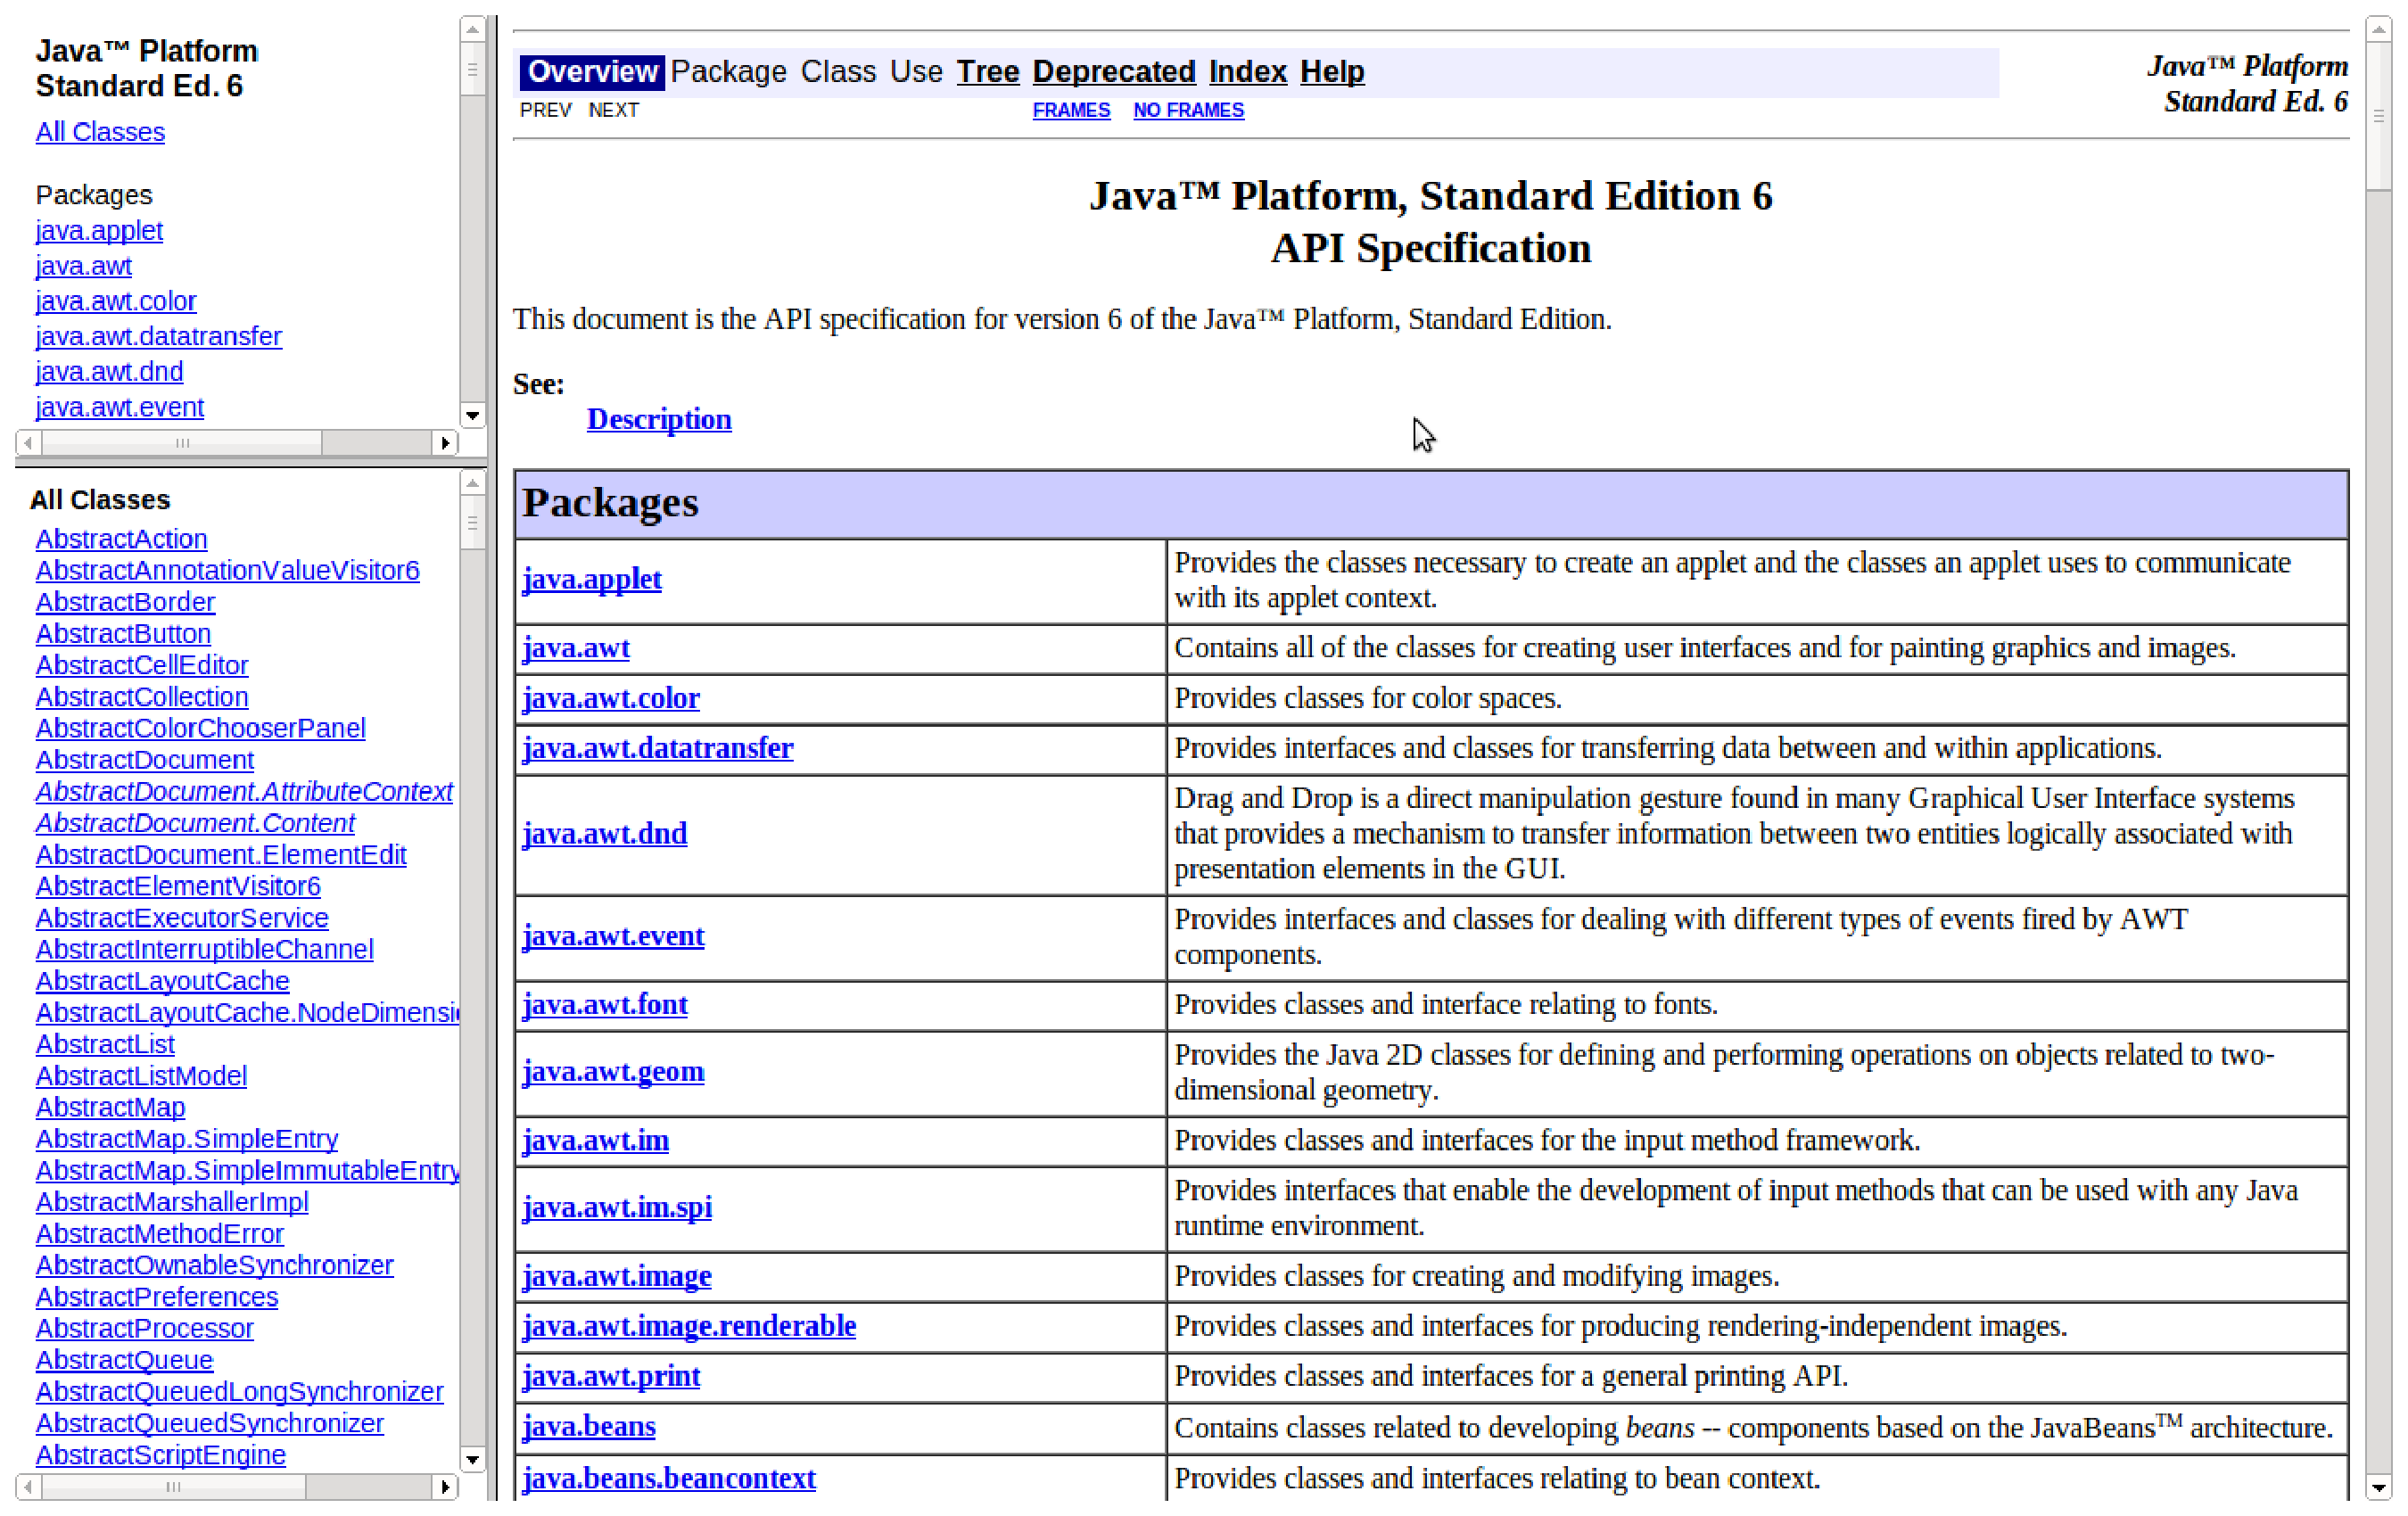
\includegraphics[width=\textwidth]{gfx/javadoc}
  \caption{The Java API main page}
  \label{fig:ajavadoc}
\end{figure}

You can see that there are three frames: top-left, a list of packages
(we will learn what packages are at a later point); bottom-left, a
list of classes; right, the main frame. You can find a lot of
information about all classes in the Java Library on this website. You
can also get a local copy if you plan to work without an internet
connection. 

Look up any class (e.g.~String) in the list of classes at the
bottom-left. Click on it. Read the documentation on the main
frame. Every page in Java Doc follows the same structure: 

\begin{description}
\item[General description: ] at the beginning.
\item[List of fields: ] all visible fields of the class, if any.
\item[List of constructor methods: ] each of them with a brief
  description, a list of parameters and other useful information, and
  a link to a more detailed description.
\item[List of methods: ] each of them with a brief
  description, a list of parameters and other useful information, and
  a link to a more detailed description.
\item[Detailed description of methods. ] 
\end{description}

You must become familiar with the Java Doc. You will use it very often
as a Java programmer. 

\subsection{A new type of loop: do\ldots while}
\label{sec:new-type-loop}

With a loop you can perform the same operations over and over
again. However, if the condition for the loop is never true a
\texttt{while} loop will never run; and sometimes you need it to run
at least once, like in this case:

\begin{verbatim}
    println "Enter the names of your friends. Finish by typing END."
    String name = System.console().readLine()
    println s + ": friend"
    while (s != "END") {
      println s + ": friend"
      name = System.console().readLine()
    }
\end{verbatim}

In this brief example you need to repeat the same code to read input
from the user in two different places. If
the only way to do loops was using \texttt{while}, this repetition
could not be avoided (and in a less trivial program, with
intelligent error-checking and the like, this could be a lot of
repetition!). Fortunately, we can use a \texttt{do\ldots while} loop: 

\begin{verbatim}
    println "Enter the names of your friends. Finish by typing END."
    do {
      String name = System.console().readLine()
      println s + ": friend"
    } while (s != "END")
\end{verbatim}


Remember, repeated code is usually a bad sign: a symptom of poor
design and/or poor programming. When you have the same code in two
different places, and make a change in one of them, it is very easy to
forget to change the other too\ldots a common source of bugs for
careless programmers. If you notice you have repeated code in your
program, think twice about a better way of doing things, without
repetition. There is a general principle in programming usually
referred to as DRY: \textbf{Don't Repeat Yourself}. Keep it in mind at
all times.


\subsubsection*{Exercise}

Make a class that implements a method 
that reads a list of marks between 0 and 100 from the
user, one per line, and stops when the user introduces a -1. The
program should output at the end (and only at the end) how many marks
there were in total, how many were distinctions (70--100), how many
were passes (50--69), how many failed (0--49), and how many were
invalid (e.g. 150 or -3). Use \texttt{readLine()} exactly once.

\subsubsection{Casting: conversion of simple types}
\label{sec:cast-conv-simple}

As you already know, Groovy is a dynamically-typed language, which
means that a variable can change its type during the execution of the
program (the box can change its \emph{type} tag). 

Java, on the other hand, is a statically-typed language. Once a
variable is created, Java will not change its type. If you try to
assign it a value of a different type it will complain.

And yet there are times in which you have an \verb+int+ but want to
transform it into a \verb+double+ to perform division, or some other
similar situation. This what \emph{casting} is for. When you cast a
variable you change its type, as in the following example: 

\begin{verbatim}
    int i = 1;
    double d = (int) i;
\end{verbatim}

This code will take the value of \verb+i+, which is 1, and transform
it into a double (\verb+1.0+) before assigning it to the
variable \verb+d+. 

Note that not all castings can be done transparently. If you cast a
\verb+double+ into an \verb+int+, for example, you will lose the
decimal part because there is no decimal part in an \verb+int+. 

\paragraph{Casting for complex types?}
\label{sec:cast-compl-types}

There is also a version of casting for complex types, but it is more
complicated and is related to type hierarchies. We will see how it
works when the time is due.

\subsection{Strings and chars}
\label{sec:strings-chars}

In Groovy, you could use either single quotes or double quotes to mark
a String. In Java you can only use the latter. Single quotes are used
to mark values of type \verb+char+. 

\begin{verbatim}
    // a one-character String in Groovy, 1 char in Java
    char c     = 'a';               

    // a String in both languages
    String str = "This is a string";

    // the following is valid in Groovy, but invalid in Java
    String s2  = 'Another string';  
\end{verbatim}

\subsection{A new complex type: Arrays}
\label{sec:arrays}

A String can be seen as a series of characters one after the
other. The idea can be extended to think of series of other simple
types, not just chars but also integers and doubles. This is called an
\emph{array}. 

Arrays are a way of having several elements of data of the same type;
for example, a company could have a payroll program with an array with
the IDs of all its employees (an array of integers). In Groovy and
Java, arrays can be of simple but also complex types; therefore, the
aforementioned program could also have array of Strings to store the
names of the employees. 

An array is declared using square brackets. Square brackets are also
used to access the elements in the array. Let's see an example: 

\begin{verbatim}
    int[] employeeIdArray;
    employeeIdArray = new Array[5]();
    employeeIdArray[0] = 123;
    employeeIdArray[1] = 55;
    employeeIdArray[2] = 14;
    employeeIdArray[3] = 642;
    employeeIdArray[4] = 243;
    println "Out first employee has ID:" + employeeIdArray[0];
    println "Our company has " + employeeIdArray.length + " employees";
\end{verbatim}

As you can see, sometimes you need a number inside the brackets and
sometimes you do not. You do not need a number to declare the array,
i.e.~to tell the computer that you want to have an array (of integers,
in this case). As all declarations, this reserves a box of type
``array of integers, int[]'' and name \verb+employeeIdArray+. In the
next line, we reserve a portion of memory to store the actual
integers, and of course we have to specify the length; otherwise
\verb+new+ will not know how much memory to allocate. Finally, when we
want to access an element in an array, either for reading or for
writing/replacing, we also have to specify \emph{which} element we
want to access. 

All arrays in Java have a field called \verb+length+ that is equal to
the size of the array. This value never changes. When an array is
created (using \verb+new+) its size is determined once and for all. 

\subsubsection*{Curly-bracket initialisation of arrays}
\label{sec:curly-brack-init}

Initialising an array element-by-element is boring and takes a lot of
space. There is a special notation using curly brackets that allows
programmers to initialise an array in one line: 

\begin{verbatim}
    int[] employeeIdArray = {123, 55, 14, 642, 243};
\end{verbatim}

If you write something like this, Java will automatically calculate
the size of the array for you and will allocate memory for it and
point to it. 

\subsubsection*{2D, 3D, and beyond\ldots}
\label{sec:2d-3d-beyondldots}

You can also have arrays of arrays, in which case they are usually
called matrices: 2-D matrices, 3-D matrices, etc. 



\subsubsection{Exercise}
\label{sec:exercisejfjfj}

Write a small program that asks for the names and IDs of all employees
in a small company, and store them in an array of integers and an
array of Strings. The company has 10 employees.

Use a loop to go through both arrays and print the names and IDs of
those employees whose ID is less than 1000. Use another loop to print
the names and IDs of those employees whose name starts with ``J''
or~``S''. 



%%% Local Variables:
%%% mode: latex
%%% TeX-master: "main"
%%% End:
